\documentclass[a4,useAMS,usenatbib,usegraphicx]{latex/mn2e} 
%\documentclass{latex/emulateapj} 
%External Packages and personalized macros
%=========================================================================
%		EXTERNAL PACKAGES
%=========================================================================
\usepackage{amsmath} 
\usepackage{amssymb} 
\usepackage[section]{placeins}
\usepackage {graphicx}
%\usepackage{graphics}
\usepackage[dvips]{epsfig}
\usepackage{epsfig}  
\usepackage{color}
\usepackage[normalem]{ulem}
\usepackage{hyperref}
\usepackage{caption}
%Non reposionated tables
\usepackage{float}
\restylefloat{table}

%=========================================================================
%		INTERNAL MACROS
%=========================================================================
\def\be{\begin{equation}}
\def\ee{\end{equation}}
\def\ba{\begin{eqnarray}}
\def\ea{\end{eqnarray}}

% To highlight comments 
\definecolor{red}{rgb}{1,0.0,0.0}
\newcommand{\red}{\color{red}}
\definecolor{darkgreen}{rgb}{0.0,0.5,0.0}
\newcommand{\SRK}[1]{\textcolor{darkgreen}{\bf SRK: \textit{#1}}}
\newcommand{\SRKED}[1]{\textcolor{darkgreen}{\bf #1}}

\newcommand{\LCDM}{$\Lambda$CDM~}
\newcommand{\beq}{\begin{eqnarray}}  
\newcommand{\eeq}{\end{eqnarray}}  
\newcommand{\zz}{$z\sim 3$} 
\newcommand{\apj}{ApJ}  
\newcommand{\apjs}{ApJS}  
\newcommand{\apjl}{ApJL}  
\newcommand{\aj}{AJ}  
\newcommand{\mnras}{MNRAS}  
\newcommand{\mnrassub}{MNRAS accepted}  
\newcommand{\aap}{A\&A}  
\newcommand{\aaps}{A\&AS}  
\newcommand{\araa}{ARA\&A}  
\newcommand{\nat}{Nature}  
\newcommand{\physrep}{PhR}
\newcommand{\pasp}{PASP}    
\newcommand{\pasj}{PASJ}    
\newcommand{\avg}[1]{\langle{#1}\rangle}  
\newcommand{\ly}{{\ifmmode{{\rm Ly}\alpha}\else{Ly$\alpha$}\fi}}
\newcommand{\hMpc}{{\ifmmode{h^{-1}{\rm Mpc}}\else{$h^{-1}$Mpc }\fi}}  
\newcommand{\hGpc}{{\ifmmode{h^{-1}{\rm Gpc}}\else{$h^{-1}$Gpc }\fi}}  
\newcommand{\hmpc}{{\ifmmode{h^{-1}{\rm Mpc}}\else{$h^{-1}$Mpc }\fi}}  
\newcommand{\hkpc}{{\ifmmode{h^{-1}{\rm kpc}}\else{$h^{-1}$kpc }\fi}}  
\newcommand{\hMsun}{{\ifmmode{h^{-1}{\rm {M_{\odot}}}}\else{$h^{-1}{\rm{M_{\odot}}}$}\fi}}  
\newcommand{\hmsun}{{\ifmmode{h^{-1}{\rm {M_{\odot}}}}\else{$h^{-1}{\rm{M_{\odot}}}$}\fi}}  
\newcommand{\Msun}{{\ifmmode{{\rm {M_{\odot}}}}\else{${\rm{M_{\odot}}}$}\fi}}  
\newcommand{\msun}{{\ifmmode{{\rm {M_{\odot}}}}\else{${\rm{M_{\odot}}}$}\fi}}  
\newcommand{\lya}{{Lyman$\alpha$~}}
\newcommand{\clara}{{\texttt{CLARA}}~}
\newcommand{\rand}{{\ifmmode{{\mathcal{R}}}\else{${\mathcal{R}}$ }\fi}}  
%SAMPLES
\newcommand{\GHBDM}{\texttt{GH}$_{\mbox{\tiny{BDM}}}$ }
\newcommand{\GHFOF}{\texttt{GH}$_{\mbox{\tiny{FOF}}}$ }
\newcommand{\IHBDM}{\texttt{IH}$_{\mbox{\tiny{BDM}}}$ }
\newcommand{\IHFOF}{\texttt{IH}$_{\mbox{\tiny{FOF}}}$ }
\newcommand{\PBDM}{\texttt{P}$_{\mbox{\tiny{BDM}}}$ }
\newcommand{\PFOF}{\texttt{P}$_{\mbox{\tiny{FOF}}}$ }
\newcommand{\IPBDM}{\texttt{IP}$_{\mbox{\tiny{BDM}}}$ }
\newcommand{\IPFOF}{\texttt{IP}$_{\mbox{\tiny{FOF}}}$ }
\newcommand{\RIPBDM}{\texttt{RIP}$_{\mbox{\tiny{BDM}}}$ }
\newcommand{\RIPFOF}{\texttt{RIP}$_{\mbox{\tiny{FOF}}}$ }


%MY COMMANDS #############################################################
\newcommand{\sub}[1]{\mbox{\scriptsize{#1}}}
\newcommand{\dtot}[2]{ \frac{ d #1 }{d #2} }
\newcommand{\dpar}[2]{ \frac{ \partial #1 }{\partial #2} }
\newcommand{\pr}[1]{ \left( #1 \right) }
\newcommand{\corc}[1]{ \left[ #1 \right] }
\newcommand{\lla}[1]{ \left\{ #1 \right\} }
\newcommand{\bds}[1]{\boldsymbol{ #1 }}
\newcommand{\oiint}{\displaystyle\bigcirc\!\!\!\!\!\!\!\!\int\!\!\!\!\!\int}
\newcommand{\mathsize}[2]{\mbox{\fontsize{#1}{#1}\selectfont $#2$}}
\newcommand{\eq}[2]{\begin{equation} \label{eq:#1} #2 \end{equation}}
\newcommand{\lth}{$\lambda_{th}$ }
%#########################################################################

\begin{document}

%=========================================================================
%		FRONT MATTER
%=========================================================================
\title{Analysis of bulk void regions}
\author[S. Bustamante and J.E. Forero-Romero]{
\parbox[t]{\textwidth}{\raggedright 
  Sebastian Bustamante \thanks{sbustama@pegasus.udea.edu.co}$^{1}$ 
  Jaime E. Forero-Romero$^{2}$ 
}
\vspace*{6pt}\\
$^1$Instituto de F\'{\i}sica - FCEN, Universidad de Antioquia, Calle
67 No. 53-108, Medell\'{\i}n, Colombia\\ 
$^2$Departamento de F\'{i}sica, Universidad de los Andes, Cra. 1
No. 18A-10, Edificio Ip, Bogot\'a, Colombia
}

\maketitle

\begin{abstract}


\end{abstract}

\begin{keywords}
Cosmology: large-scale Structure of Universe, 
galaxies: star formation - line: formation
\end{keywords}


%=========================================================================
%		PAPER CONTENT
%=========================================================================

%*************************************************************************
\section{Introduction}
\label{sec:introduction}
%*************************************************************************


The spatial distribution of galaxies describes a web-like pattern, the 
so-called cosmic web. Today it is understood that such configuration is 
driven by gravitational instabilities. ...

Relevant information about previous works and current state of the art.


%*************************************************************************
\section{The Simulation}
\label{sec:the_simulation}
%*************************************************************************


As it was previously mentioned, we use an unconstrained cosmological 
simulation, the Bolshoi simulation, to identify the possible large scale 
environment of the Local Group. This is a similar approach to the one already 
used by \SRKED{[reference here]}.



The Bolshoi simulation follows the non-linear evolution of a dark matter 
density field on a cubic volume of size $250$\hMpc sampled with $2048^3$ 
particles. The cosmological parameters in the simulation are 
$\Omega_{\rm m}=0.27$, $\Omega_{\Lambda}=0.73$, $h=0.70$, $n=0.95$ and 
$\sigma_{8}=0.82$ for the matter density, cosmological constant, 
dimensionless Hubble parameter, spectral index of primordial density 
perturbations and normalization for the power spectrum. The mass of each 
particle in the simulation is $m_{\rm p}=1.4\times 10^{8}$\hMsun.
We identify halos with two algorithms, the Friends-of-Friends \SRKED{
[reference here]} algorithm and the Bound Density Maximum algorithm.




%*************************************************************************
\section{Algorithms to quantify the cosmic web}
\label{sec:algorithms_cosmic_web}
%*************************************************************************



%-------------------------------------------------------------------------
\subsection{The tidal web (T-web)}
\label{subsec:Tweb}
%-------------------------------------------------------------------------



The first algorithm  we use to identify the cosmic web is based upon the
diagonalization of the tidal tensor, defined as the Hessian of a 
normalized gravitational potential  


%.........................................................................
%Tidal Tensor
\begin{equation}
T_{\alpha\beta} = \frac{\partial^2\phi}{\partial x_{\alpha}\partial x_{\beta}}
\end{equation}
%.........................................................................
where the physical gravitational potential has been rescaled by a factor 
$4\pi G\bar{\rho}$ in such a way that $\phi$ satisfies the following 
equation



%.........................................................................
%Poisson
\begin{equation}
\nabla^2\phi = \delta,
\end{equation}
%.........................................................................
where $\bar{\rho}$ is the average density in the Universe, $G$ is the 
gravitational constant and $\delta$ is the dimensionless matter 
overdensity.



%-------------------------------------------------------------------------
\subsection{The velocity  web (V-web)}
\label{subsec:Vweb}
%-------------------------------------------------------------------------



We also use a kinematical method to define the cosmic-web environment in 
the simulation. The method has been thoroughly described in XXX and 
applied to study the shape and spin alignment in the Bolshoi simulation 
here XX. We refer the reader to these papers to find a detailed 
description of the algorithm, its limitations and capabilities. Here we 
summarize the most relevant points for the discussion. 



The V-web method for environment finding is based on the local shear 
tensor calculated from the smoothed DM velocity field in the simulation.
The central quantity is the following dimensionless quantity 


%.........................................................................
%V-Web Definition
\eq{V_web}
{
\Sigma_{\alpha\beta} = -\frac{1}{2H_0}\pr{\frac{\partial v_{\alpha}}
{\partial x_{\beta}}+\frac{\partial v_{\beta}}{\partial x_{\alpha}}}
}
%.........................................................................
where $v_{\alpha}$ and $x_{\alpha}$ represent the $\alpha$ component of 
the comoving velocity and position, respectively. $\Sigma_{\alpha\beta}$ 
can be represented by a $3\times 3$ symmetric matrix with real values,
that ensures that is possible to diagonalize and obtain three real 
eigenvalues $\lambda_{1} > \lambda_{2}>\lambda_3$ whose sum (the trace of
$\Sigma_{\alpha\beta}$) is proportional to the divergence of the local 
velocity field smoothed on the physical scale ${\mathcal R}$. 



The relative strength of the three eigenvalues with respect to a threshold
value $\lambda_{th}$ allows for the local classification of the matter 
distribution into four web types: voids, sheets, filaments and peaks, 
which correspond to regions with 3, 2, 1 or 0 eigenvalues with values 
larger than $\lambda_{th}$. Below we shall discuss a novel approach to 
define an adequate threshold value based on the visual impression of void
regions, furthermore we study other possible values based on other visual
features of the cosmic web.



%-------------------------------------------------------------------------
\subsection{The cosmic web in Bolshoi}
\label{subsec:web_in_simulations}
%-------------------------------------------------------------------------



Both established schemes to quantify the cosmic web depend on continuous 
and smooth physical quantities, i.e the peculiar velocity field and the 
density field. To calculate these quantities, a discretization over the 
volume of the simulation is performed, so all the properties are reduced 
to single values associated to discrete cells. According to this, we 
divide the overall volume into $(256)^3$ cells, so each cell has an 
associated comoving cubic volume of $0.98 \mbox{ Mpc h}^{-1}$. Finally, in 
order to reduce possible effects due to the discretization process, a 
gaussian softening is performed between neighbour cells.



Once defined the numerical details about both classification schemes, we
shall analyse the dependence on the threshold value $\lambda_{th}$ for 
each one. For this, we shall use the distribution of dark matter halos as 
tracer of the underlying matter field in order to be more consistent with
available observational data. In the figure \ref{fig:halos_fractions} we 
calculate fractions of halos within each one of the defined environments 
based upon the FOF catalogue of the simulation and for an extensive \lth 
range. Then we look for some key feature that could indicated us a 
possible optimal value of the \lth value. One first step forward our quest 
is the behaviour of the V-web scheme compared with the T-web. As was 
previously established by \SRKED{Hoffman et al. (2012)} and as can be seen 
in the figure \ref{fig:halos_fractions}, V-web scheme is significantly more
sensible to variations of the $\lambda_{th}$ value, since all fractions of
halos for the V-web change significantly in the range $[0,0.4]$, whereas, 
for the T-web scheme, fractions change smoothly throughout all \lth range 
covered. From this, it is then expected that the optimal \lth value for 
the V-web scheme is less than the T-web value.



The more notorious characteristic of the figure \ref{fig:halos_fractions} 
is the behaviour of the fraction of halos within sheet regions for both 
web schemes, increasing until a local maximum, and then decreasing. The 
increasing or decreasing rate of the fraction of halos for some region 
could be interpreted as a measure of the degree of non-linearity of such 
region for some specific \lth value. For example, filaments and knots, 
that are the most non-linear regions of the universe, have a negative rate
for all covered \lth range. In the case of voids, the situation is 
completely opposite, where fractions of halos increase in everywhere. If 
we think in terms of the underlying matter field of the cosmic web, \lth 
is just a cutting parameter between high non-linear regions (filament and 
knots) and low non-linear (voids and sheets). Furthermore, if we take into 
account that dark matter halos are much more likely to form in high 
non-linear regions, it is expected the obtained behaviour of fractions of 
halos for voids, filaments and knots as we increase the \lth value. 
However, the behaviour of the fraction of halos in sheets is less clear,
increasing for low \lth values (like voids) and decreasing for higher \lth 
values (like filaments and knots). This indicates us the transitional 
character of sheet regions in the cosmic web. Our proposal here is to 
select as optimal \lth the value where the fraction of sheets reaches a
local maximum, so sheets are completely taken as intermediate transitional 
and neutral zones regarding the degree of non-linearity. According to this,
we find for the T-web scheme an optimal value $\lambda_{opt}^T = 0.36$ and
for the V-web scheme $\lambda_{opt}^V = 0.20$. In the figure 
\ref{fig:visual_impression} we show the visual impression of the cosmic 
web along with the density field for different \lth values including the 
optimal values. It can be noticed that the optimal values found reproduce 
well the visual impression.



As we have taken halos as tracers of the cosmic web, we analyse 
distributions of mass and peculiar velocity in order to assign typical 
values to each type of environment. In the figure 
\ref{fig:typical_mass_velocity} we calculate both distributions for web 
schemes and using the FOF catalogue of the simulation. Thick lines 
correspond to the median of the distribution and filled regions limited by
dashed lines correspond to quartiles $Q_1$ and $Q_3$, it means, $50\%$ of
all halos are within such regions for every \lth value and for each type 
of environment. We rather use median and quartiles as measure of 
dispersion because there are some very unusual and extreme values that 
makes the usual analysis based upon means and standard deviations less 
reliable.



A first interesting feature of the figure  \ref{fig:typical_mass_velocity} 
is the median mass for each region. In the case of the T-web, although 
dispersions of the distribution of mass for each environment are 
considerably overlapped each other, the median value is very 
well-differentiated among types of environment, indicating that it is 
possible to assign typical values of mass to each region, and being 
consistent with expectations, where low mass halos are typical in voids 
until high mass halos in knots. For the case of the V-web scheme, all
medians and dispersions are completely overlapped, specially for values 
grater than the optimal \lth value, indicating that it is not possible to
assign typical mass ranges to each environment as quantified by this 
scheme. For peculiar velocities, this situation is opposite, where V-web
scheme is much more adequate to assign typical distributions of velocity
to each environment. Although T-web also makes a differentiation in the 
distributions of velocity, this is very slight compared with the V-web 
case. These results can be explained by appealing the physical origin of 
each web scheme. As T-web is based upon the Hessian matrix of the 
potential field, it is expected all quantities related to the potential, 
like density field and distribution of halos mass, are well-differentiated 
among each region, while for the V-web scheme, based upon the shear 
velocity tensor, all dynamical quantities, as the peculiar velocity field 
and the distribution of halos velocity are alike expected to be 
well-differentiated among regions as quantified by this scheme.



Finally, we also calculate typical distributions of the density and 
peculiar velocity fields in each type of environment, obtaining completely
analogous results. Furthermore, we also use a BDM catalogue of the 
simulation, obtaining very similar conclusions.



%*************************************************************************
\section{Finding bulk voids}
\label{sec:bulk_voids}
%*************************************************************************


Following the recent growing interest in studying galaxy formation in 
low-density regions as cosmological tests, we use a simple method based on 
a FOF-like algorithm, where we build an input catalogue for the FOF method
with the coordinate of the center of every cell marked as void according 
to the web classification scheme adopted, setting a linking length to 
connect diagonal neighbour cells. Then, following the work of 
\SRKED{Forero-Romero et al. 2008}, we perform a percolation analysis in 
order to select the best threshold parameter that reduces percolation in 
cells. 


In figure \ref{fig:percolation_analysis_FOF} we show the result of our 
percolation analysis for both web schemes. In both cases, it can be 
noticed that the volume of the largest void region in the lower panel is 
minimized at $\lambda_{th} = 0$, what means that percolation is completely 
reduced for this threshold value. Regarding the number of voids, shown in 
the upper panel, the T-web scheme presents a expected behaviour, where the 
number of voids decreases with \lth as the largest void absorbs minor 
voids through percolation. For the V-web scheme, there is an anomaly 
around the optimal \lth value, where there is a considerable increment of 
the number of voids. In the figure \ref{fig:volume_distributions}, we 
calculate a distribution function of the volume of voids. First for 
$\lambda_{th}=0.0$ in the upper panel, where both schemes present similar 
distributions, although voids in the V-web scheme are slight biased 
towards middle volume, with a lower abundance for low volume regions than 
voids in the T-web scheme. Secondly, in the lower panel of this figure, we 
compute the same distribution of volumes for the optimal parameter 
previously established for both schemes. Here, it can be noticed a 
significant over-abundance of low volume voids for the V-web scheme 
compared with the T-web. As it was above-mentioned from the figure 
\ref{fig:typical_mass_velocity}, the \lth value can be associated, at 
least indirectly, to an increase of the threshold value of the peculiar 
velocity field, in the case of the V-web, or the density field for the 
T-web. Therefore, the over-abundance of low volume voids for the V-web 
implies high fluctuations in the peculiar velocity field, while the 
density field is more robust. In the same plot, it can be noticed a lack 
of high volume voids, what is also due to percolation, since high volume 
voids are absorbed by the largest void.


In the light of the previous results, we choose a threshold parameter 
$\lambda_{th} = 0$ for all subsequent analysis of voids in order to avoid
percolation and high fluctuations of the V-web scheme. In spite of this 
value is quite different to the previously established optimal threshold
for each scheme, bulk voids for $\lambda_{th} = 0$ are expected to be 
the central cores of bulk voids at higher threshold values, assuming that 
percolation could be reduced. Therefore, global properties of voids are 
expected to maintain for $\lambda_{th} = 0$.



%*************************************************************************
\section{Properties of voids}
\label{sec:properties}
%*************************************************************************


Once defined the proper scheme to classify bulk voids in the simulation,
we proceed to analyse their physical properties, like the inertia values,
the density and peculiar velocities profiles as calculated over the grid 
and profiles of number of halos.


%-------------------------------------------------------------------------
\subsection{Shape of voids}
\label{subsec:shape_voids}
%-------------------------------------------------------------------------


Quantifying the shape of voids is gaining importance due to cosmological 
tests such as the Alcock-Paczynski test \SRKED{Sutter, et.al (2012)}, so 
we compute here the reduced inertia tensor through the next expression in 
order to determine shape distributions of bulk voids.


%.........................................................................
%Reduced inertia tensor
\eq{ReducedIntertia}
{ \tau_{ij} = \sum_l \frac{ x_{l,i}x_{l,j}  }{R_l^2} }
%.........................................................................
where $l$ is an index associated to each cell of the current region, 
$i$ and $j$ indexes run over each spatial direction and finally 
$R_l$ is defined as $R_l^2 = x_{l,1}^2 + x_{l,2}^2 + x_{l,3}^2$. All 
positions are measured from the respective geometric center of each void.


The eigenvalues of the reduced inertia tensor, i.e. the principal moments
of inertia, are used to quantify the shape of each bulk void. They are 
denoted as $\tau_1$, $\tau_2$ and $\tau_3$ such that $\tau_1 \leq \tau_2
\leq \tau_3$. In Figure \ref{fig:distro_inertia} we show the computed
distributions for $\tau_1/\tau_2$ and $\tau_2/\tau_3$ for voids larger 
than 8 cells in order to avoid statistic fluctuations due to small regions.
We rather calculate histograms for these ratio quantities instead of each 
single value in order to avoid using an arbitrary normalization. For both 
schemes, it can be noticed that the shape distribution is completely 
spread out, thereby indicating a non-preferred geometry of void regions, 
which is in agreement with the well established high anisotropy of matter 
flows associated to this type of region. 


For a better quantification, we also perform a classification of the shape 
of voids by setting a threshold in the analysed ratio quantities. An 
anisotropic or tri-axial shape correspond to voids where $\tau_1/\tau_2 < 
0.7$ and $\tau_2/\tau_3 < 0.7$, where there is not any symmetry among the
principal directions. We find about $57.2\% \sim 61.0\%$ of total voids 
consistent with this shape, for the T-web and V-web respectively. A 
pancake or quasi-oblate shape is associated to voids where $\tau_1/\tau_2 
< 0.7$ and $\tau_2/\tau_3 > 0.7$. We found $13.1\% \sim 17.9\%$ of 
consistent voids. Filamentary or quasi-prolate voids satisfy $\tau_1/\tau_2 
> 0.7$ and $\tau_2/\tau_3 < 0.7$, with $25.4\% \sim 18.1\%$ of all voids.
Finally, isotropic or quasi-spheric voids are found when $\tau_1/\tau_2 
> 0.7$ and $\tau_2/\tau_3 > 0.7$, with $4.2\% \sim 3.1\%$ of total voids 
compatible with this shape. The threshold value of $0.7$ adopted here for
the ratios of the moments of inertia is just for illustrative purposes, 
where such distinction is rather fuzzy and continuous. However, the 
previous analysis allows us to conclude that voids are quite asymmetric 
structures.



%-------------------------------------------------------------------------
\subsection{Density profile of voids}
\label{subsec:density_voids}
%-------------------------------------------------------------------------



%*************************************************************************
\section{Conclusions}
\label{sec:conclusions}
%*************************************************************************


%*************************************************************************
\section*{Acknowledgments}  
%*************************************************************************


\bibliographystyle{mn2e}
\bibliography{references} 


%.........................................................................
%FIGURE 1: Fraction of halos in each environment
\begin{flushleft}
\begin{figure*}
\centering

  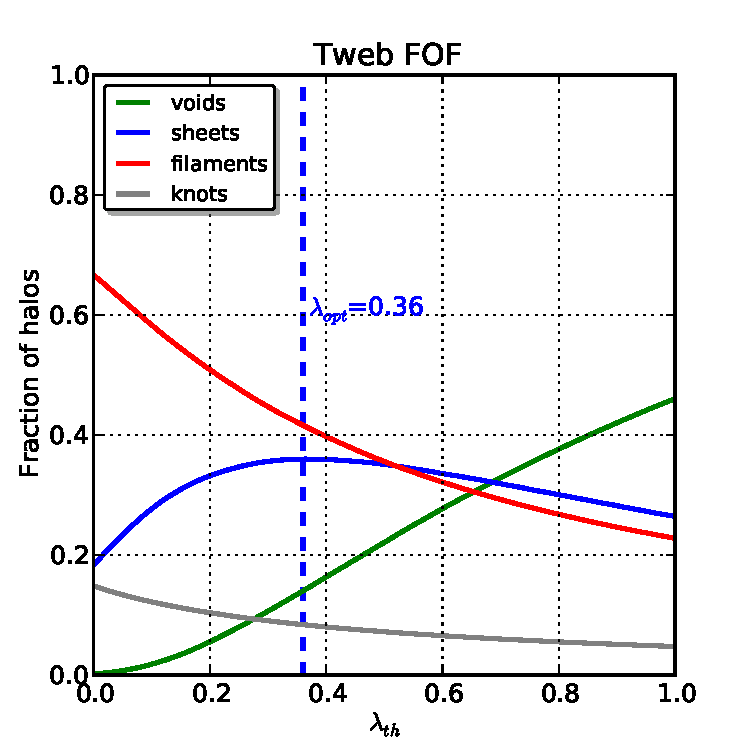
\includegraphics[trim = 0mm 0mm 5mm 5mm, clip, keepaspectratio=true,
  width=0.25\textheight]{./figures/halos_fraction_FOF_Tweb.pdf}
  
  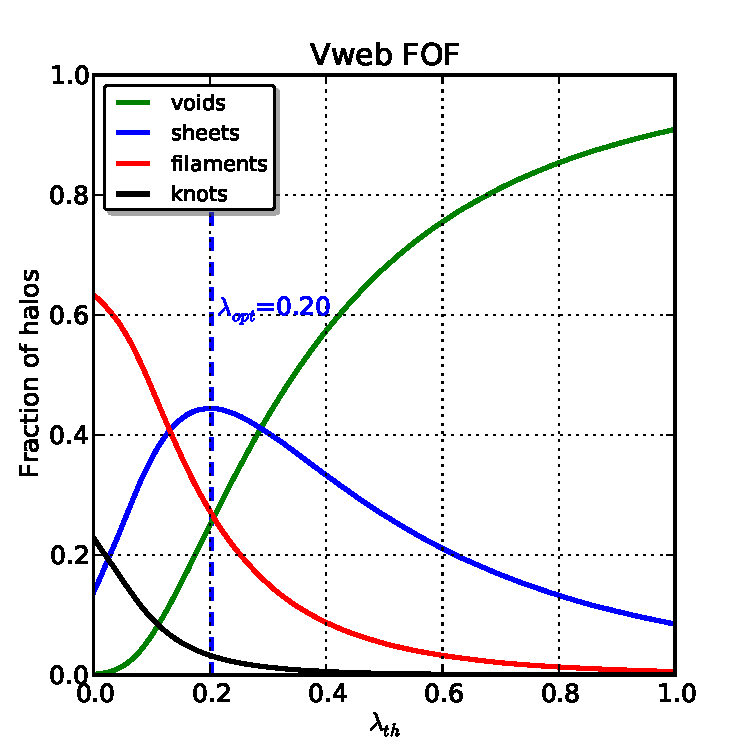
\includegraphics[trim = 0mm 0mm 5mm 5mm, clip, keepaspectratio=true,
  width=0.25\textheight]{./figures/halos_fraction_FOF_Vweb.pdf}

  \captionof{figure}{\small Fractions of halos embedded in each one of 
  the defined environments according to the \lth value. T-web scheme 
  (upper panel) and V-web scheme (lower panel). The optimal parameters 
  found are $\lambda_{opt}^{T}=0.36$ and $\lambda_{opt}^{V}=0.20$.}

  \label{fig:halos_fractions}
  \vspace{0.1 cm}

\end{figure*}
\end{flushleft}
%.........................................................................



%.........................................................................
%FIGURE 2: Visual impression of the cosmic web
\begin{flushleft}
\begin{figure*}
\centering

  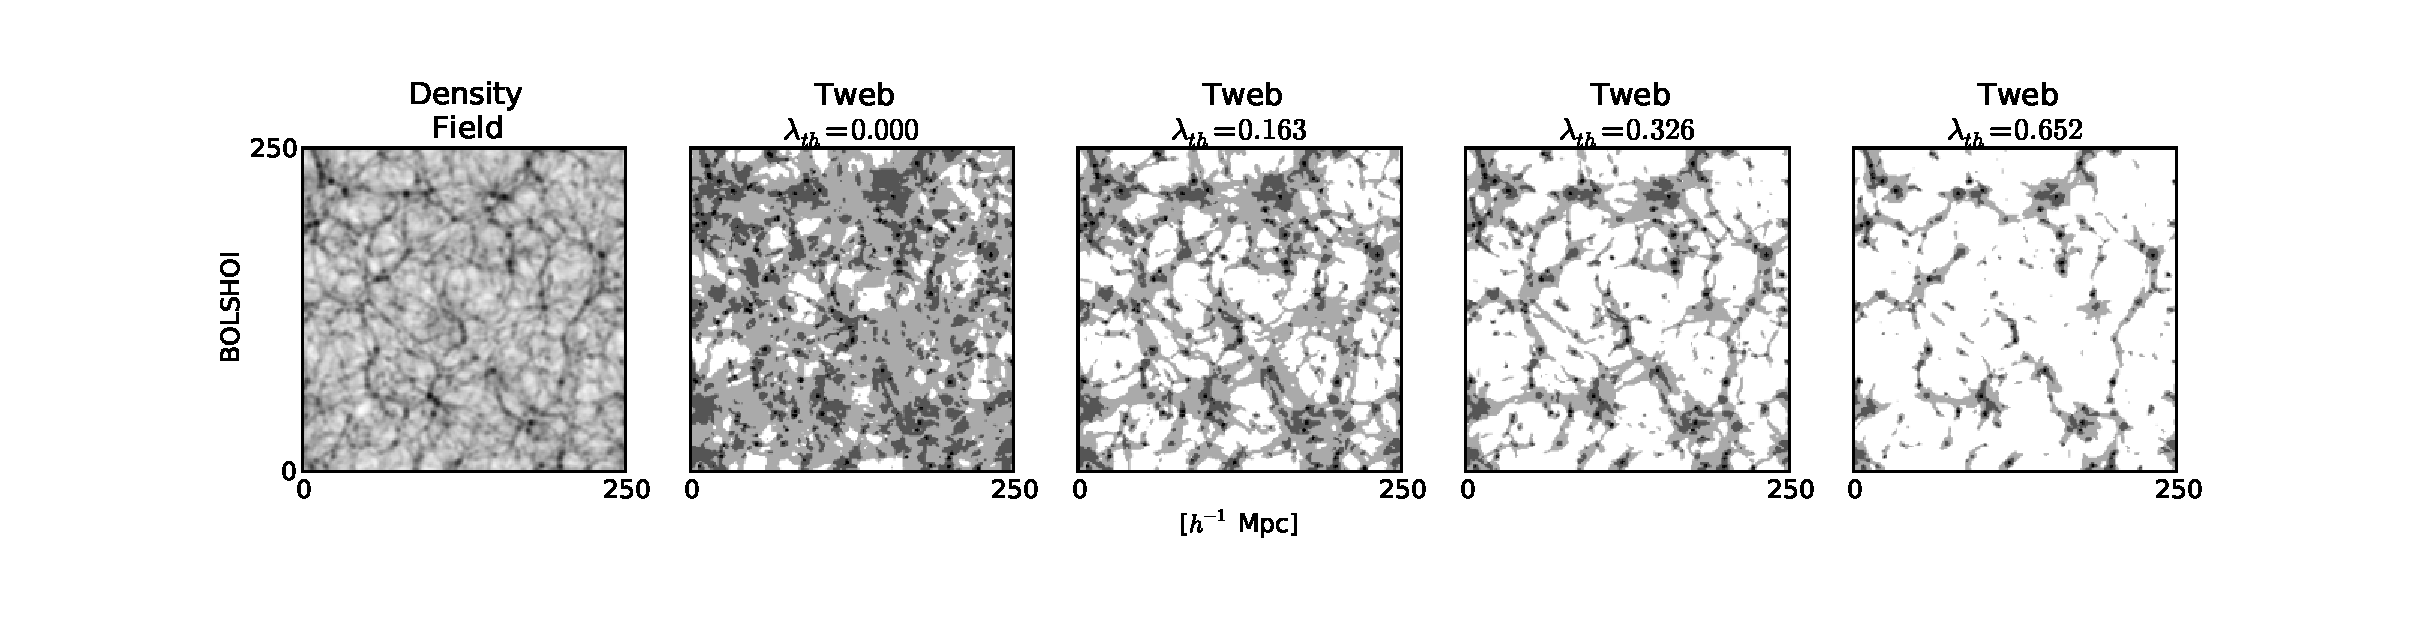
\includegraphics[trim = 42mm 10mm 37mm 10mm, clip, keepaspectratio=true,
  width=0.75\textheight]{./figures/cosmicweb_visual_Tweb.pdf}
  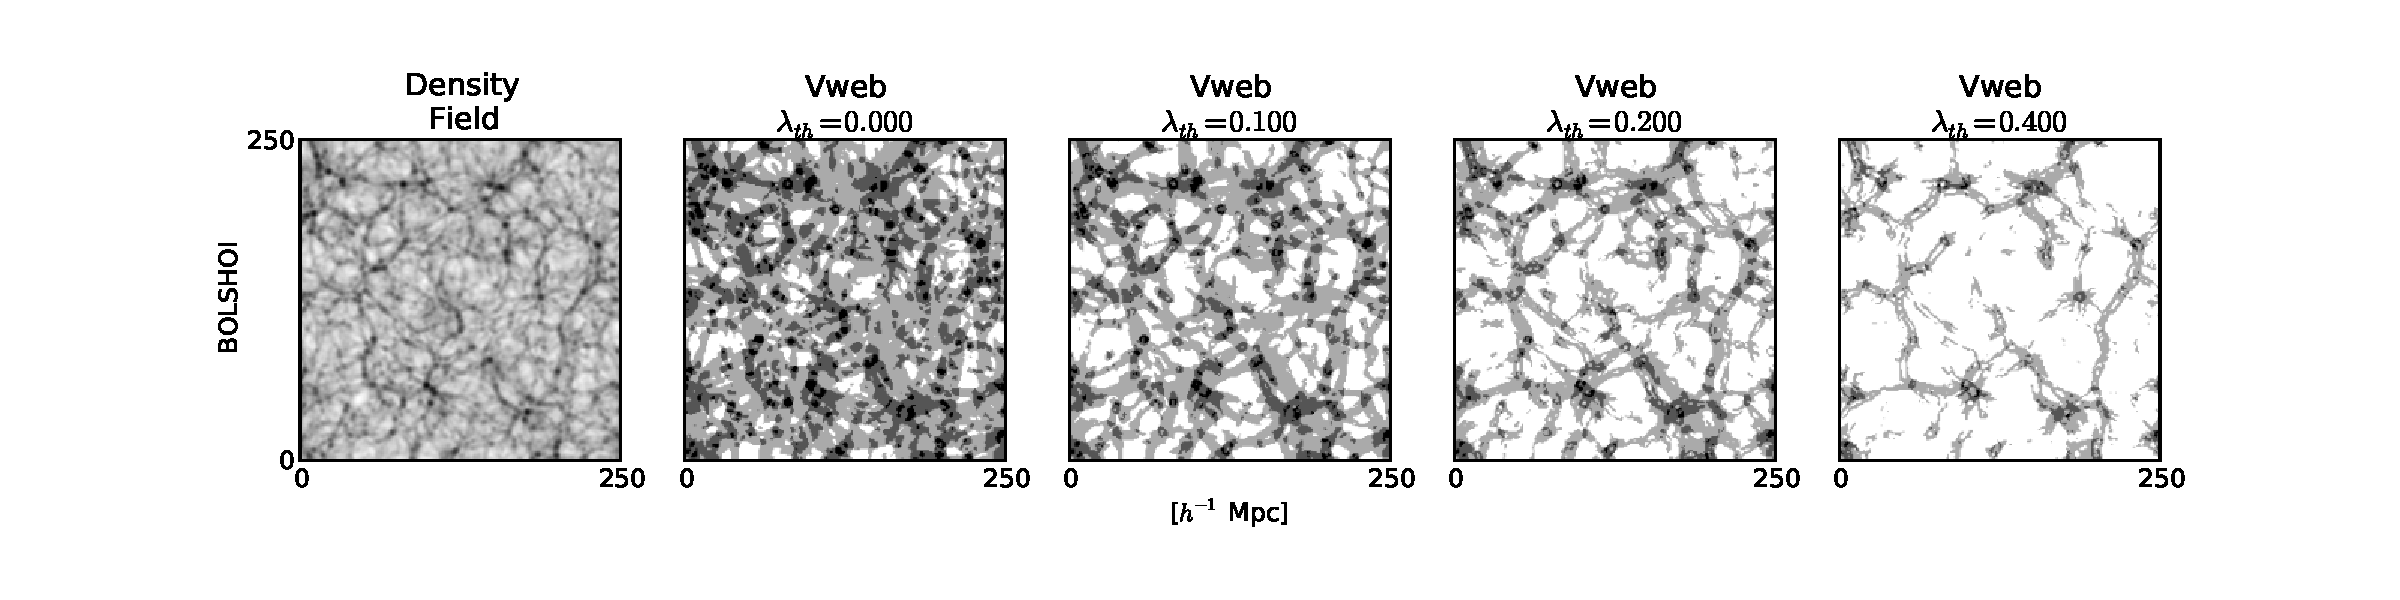
\includegraphics[trim = 42mm 10mm 37mm 10mm, clip, keepaspectratio=true,
  width=0.75\textheight]{./figures/cosmicweb_visual_Vweb.pdf}
  
  \captionof{figure}{\small Visual impression of the density field (left 
  panels), and of each classification scheme with the $\lambda_{th}$ values 
  obtained by our criteria (others panels). The color convention for each 
  environment is (white) - void, (light gray) - sheet, (gray) - filament, 
  (black) - knot. For each web scheme, it has been used the previously 
  established optimal threshold as a reference value, so plots are done 
  with the next values $\lambda_{th} = 0.0$, $\lambda_{th} = 
  \lambda_{opt}/2$, $\lambda_{th} = \lambda_{opt}$ and $\lambda_{th} = 
  2\lambda_{opt}$.}

  \label{fig:visual_impression}
  \vspace{0.1 cm}

\end{figure*}
\end{flushleft}
%.........................................................................



%.........................................................................
%FIGURE 3: Typical mass and pecular velocity
\begin{flushleft}
\begin{figure*}
\centering

  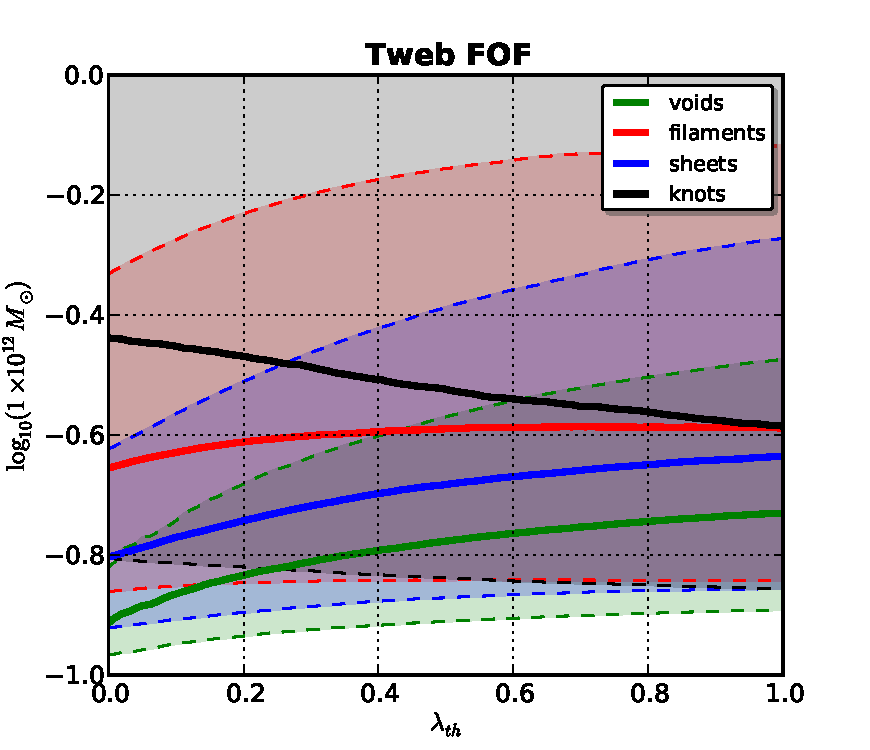
\includegraphics[trim = 0mm 0mm 0mm 0mm, clip, keepaspectratio=true,
  width=0.3\textheight]{./figures/halos_typical_mass_FOF_Tweb.pdf}
  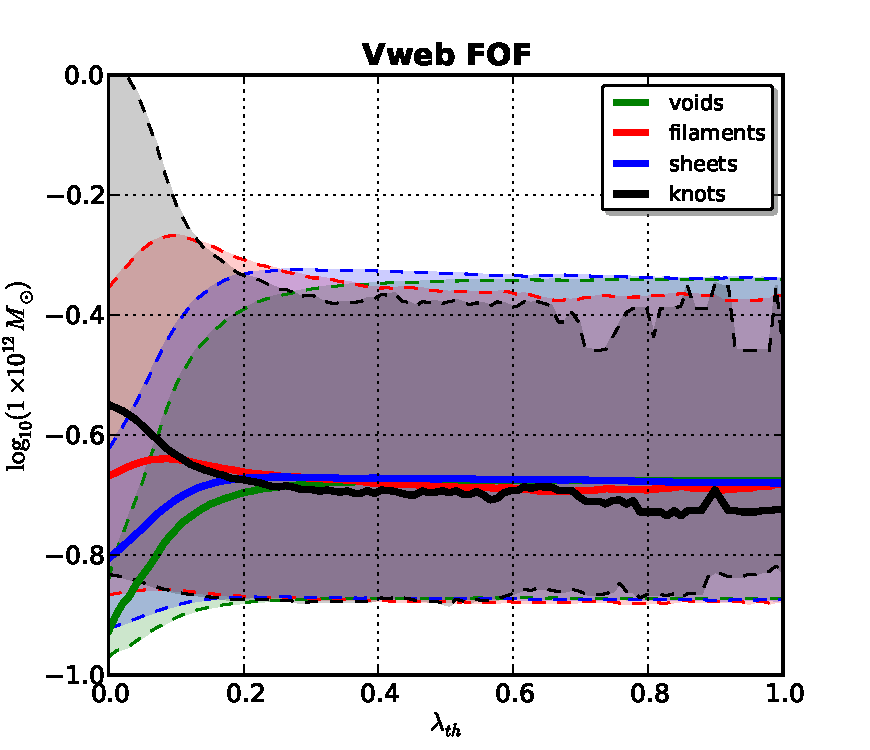
\includegraphics[trim = 0mm 0mm 0mm 0mm, clip, keepaspectratio=true,
  width=0.3\textheight]{./figures/halos_typical_mass_FOF_Vweb.pdf}  
  
  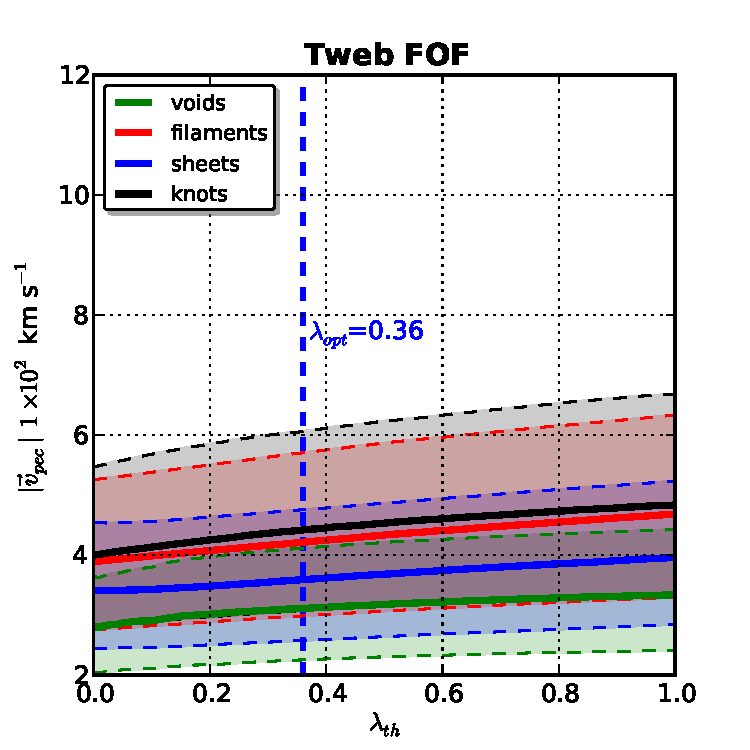
\includegraphics[trim = 0mm 0mm 0mm 0mm, clip, keepaspectratio=true,
  width=0.3\textheight]{./figures/halos_typical_velocity_FOF_Tweb.pdf}
  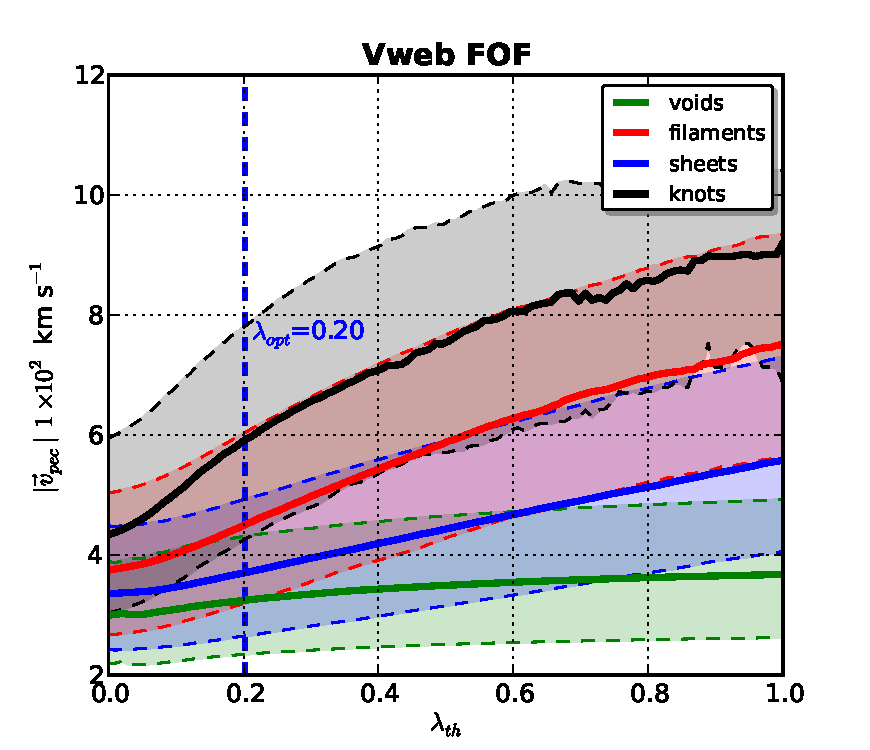
\includegraphics[trim = 0mm 0mm 0mm 0mm, clip, keepaspectratio=true,
  width=0.3\textheight]{./figures/halos_typical_velocity_FOF_Vweb.pdf}  
  
  \captionof{figure}{\small Distribution of masses of dark matter halos
  according the region where they are embedded for both web schemes 
  (upper panels) and of peculiar velocity (lower panels).}

  \label{fig:typical_mass_velocity}
  \vspace{0.1 cm}

\end{figure*}
\end{flushleft}
%.........................................................................



%.........................................................................
%FIGURE 4: Percolation analysis for FOF void finder
\begin{flushleft}
\begin{figure*}
\centering

  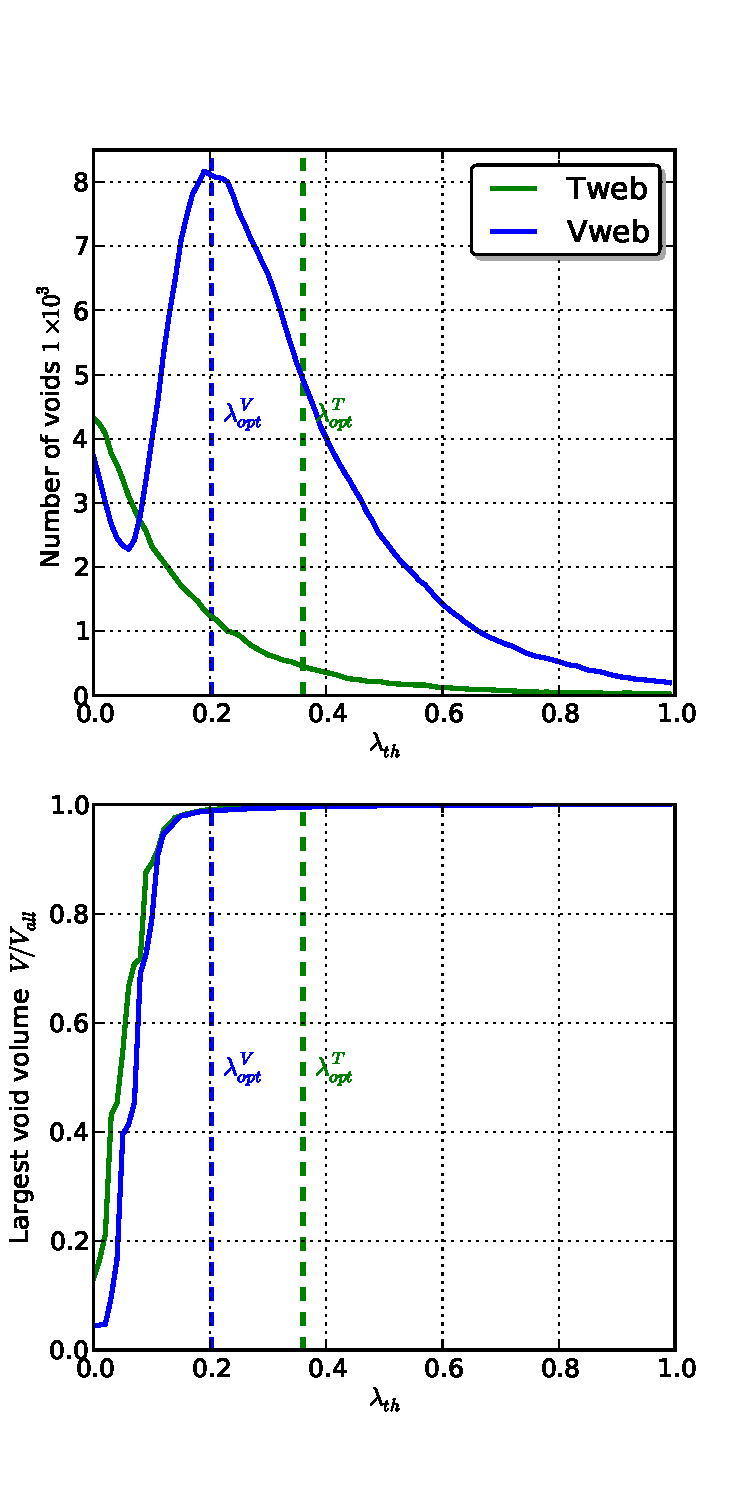
\includegraphics[trim = 1mm 10mm 8mm 18mm, clip, keepaspectratio=true,
  width=0.25\textheight]{./figures/voids_regions_percolation_FOF.pdf}

  \captionof{figure}{\small Percolation analysis of bulk void found by using
  FOF void finder algorithm. It is swept an extensive \lth range for both web
  schemes. T-web (blue lines) and  V-web (green lines). Plot of the largest 
  volume (lower panel) and the number of bulk voids found (upper panel).}

  \label{fig:percolation_analysis_FOF}
  \vspace{0.1 cm}
  
\end{figure*}
\end{flushleft}
%.........................................................................



%.........................................................................
%FIGURE 5: Volume functions of voids for null threshold and optimal threshold
\begin{flushleft}
\begin{figure*}
\centering

  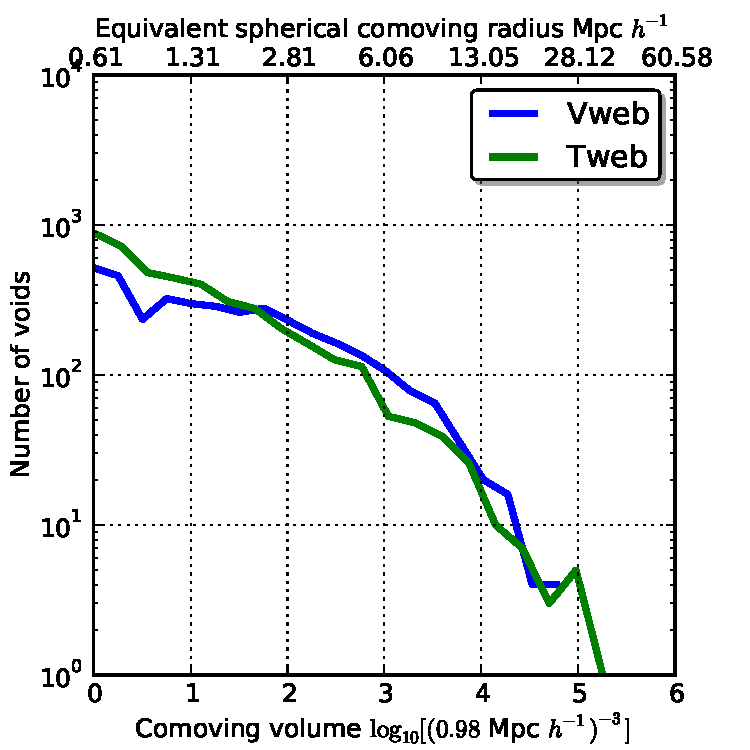
\includegraphics[trim = 0mm 0mm 5mm 0mm, clip, keepaspectratio=true,
  width=0.24\textheight]{./figures/voids_regions_volume_FOF_null.pdf}
  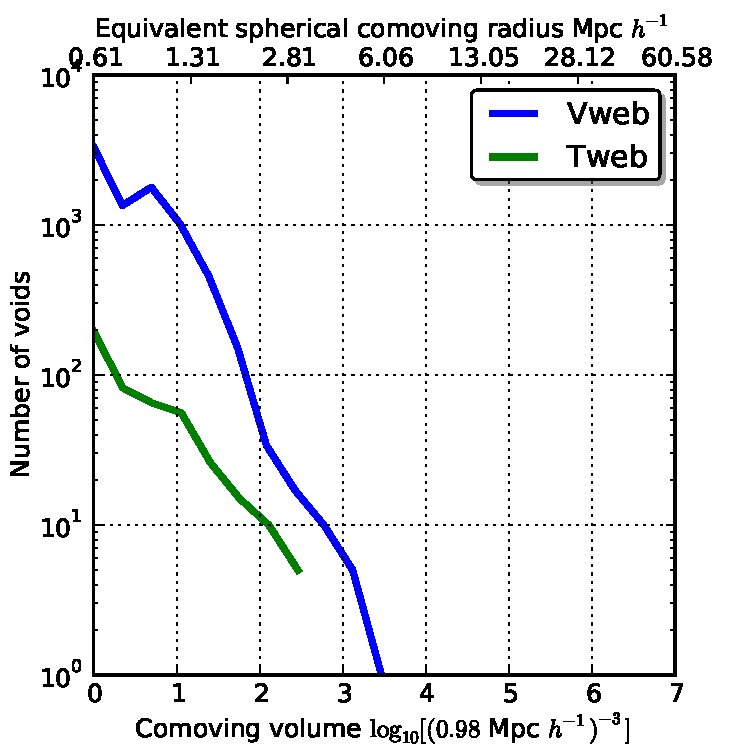
\includegraphics[trim = 0mm 0mm 5mm 0mm, clip, keepaspectratio=true,
  width=0.24\textheight]{./figures/voids_regions_volume_FOF_opt.pdf}

  \captionof{figure}{\small Volume functions of voids for both web schemes.
  In the upper panel is shown the results for the catalogue generated at
  $\lambda_{th} = 0.0$, while in the lower panel for the catalogue at 
  $\lambda_{th} = \lambda_{opt}$.}

  \label{fig:volume_distributions}
  \vspace{0.1 cm}
  
\end{figure*}
\end{flushleft}
%.........................................................................



%.........................................................................
%FIGURE 6: Distribution of eigenvalues of the inertia tensor
\begin{flushleft}
\begin{figure*}
\begin{center}

  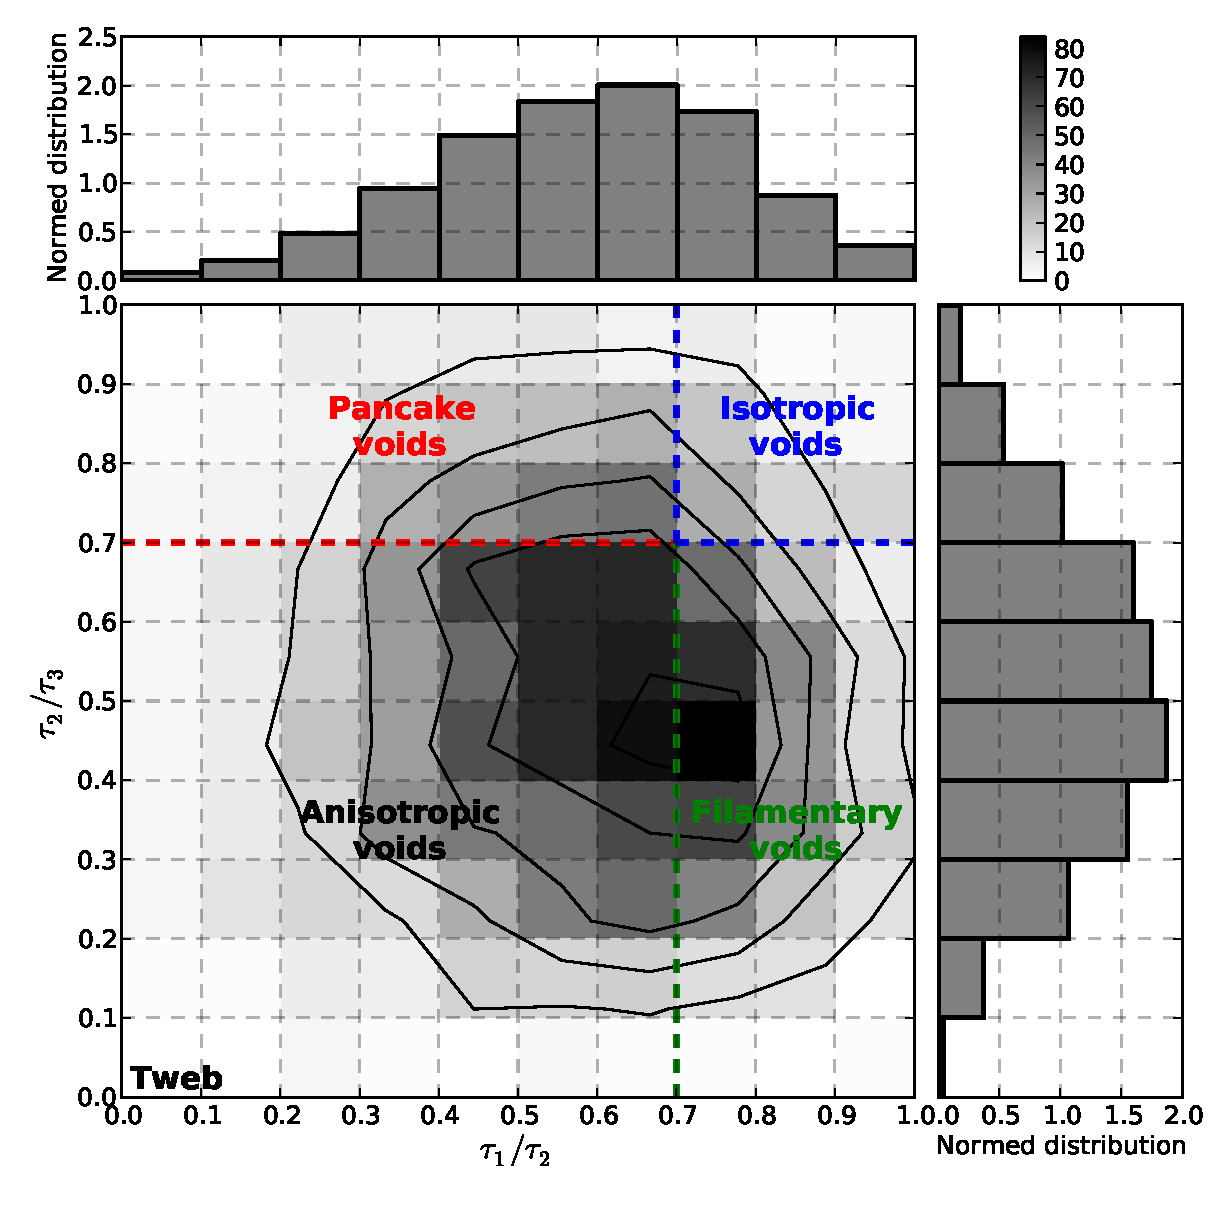
\includegraphics[trim = 7mm 9mm 1mm 0mm, clip, keepaspectratio=true,
  width=0.36\textheight]{./figures/voids_inertia_tensor_Tweb}
  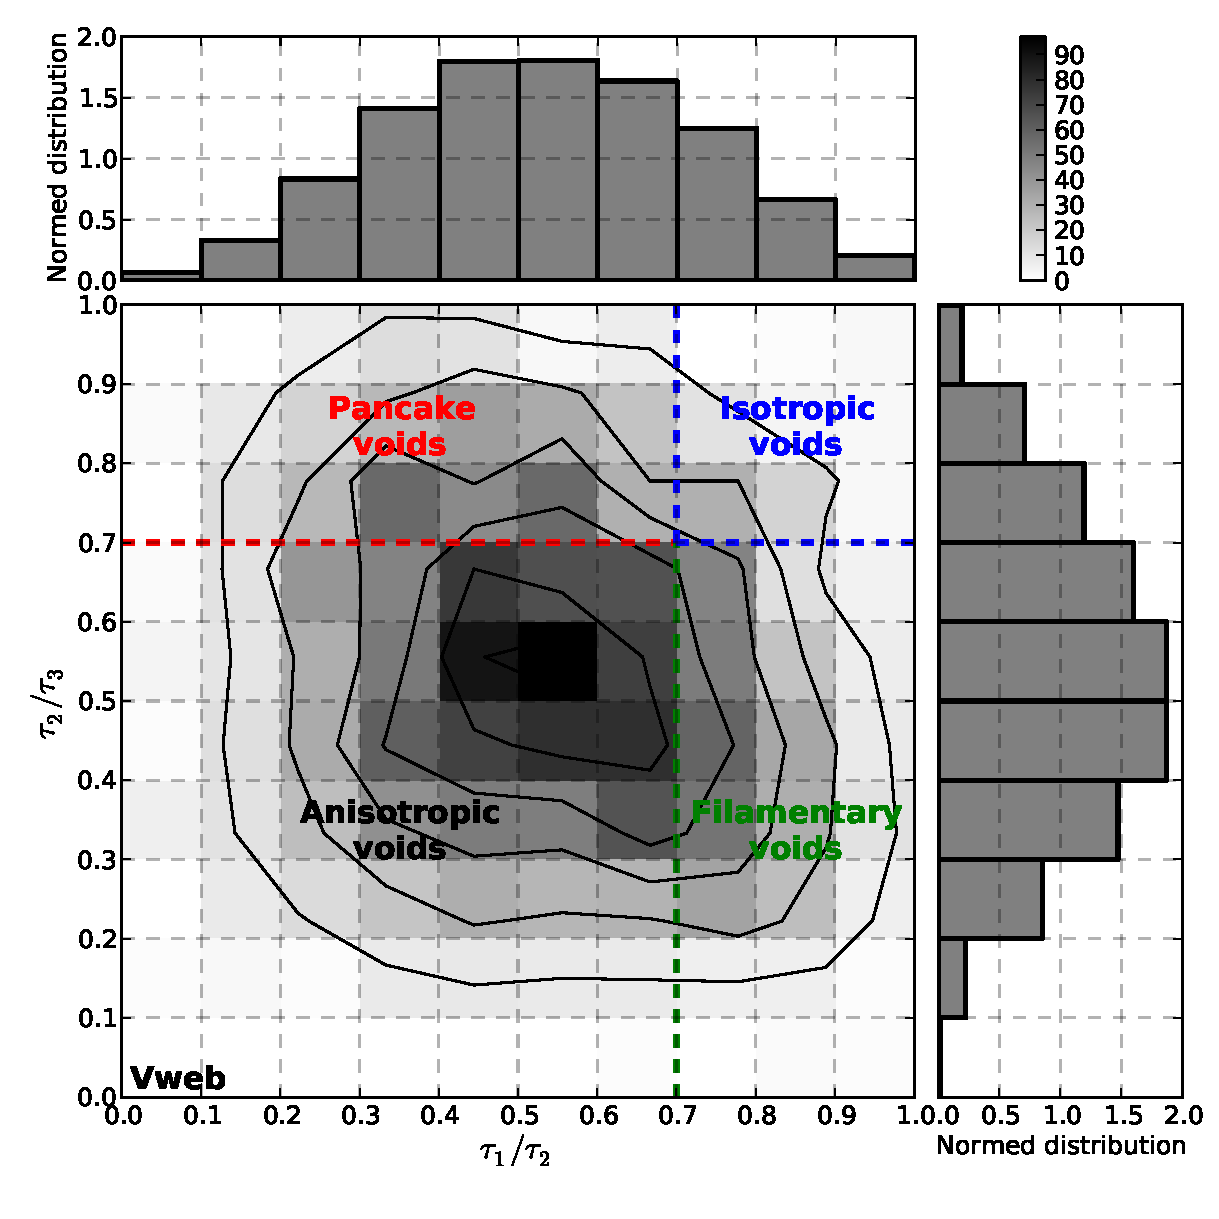
\includegraphics[trim = 7mm 9mm 1mm 0mm, clip, keepaspectratio=true,
  width=0.36\textheight]{./figures/voids_inertia_tensor_Vweb}

  \captionof{figure}{\small Histogram of eigenvalue ratio $\tau_1/\tau_2$
  vs $\tau_2/\tau_3$ for the inertia tensor of void regions. T-web 
  (upper panel) and V-web (lower panel). Number of cells per 
  region in 2D histograms are indicated by the respective colour bar. 
  Upper ($\tau_1/\tau_2$) and right ($\tau_2/\tau_3$) panels of each 
  figure shows a normalized histogram of each ratio parameter. The 
  adopted division for quantify the morphology of void regions is not
  well justified, it should be understood as a fuzzy and continuous 
  limit, done just for illustrative purposes.}

  \label{fig:distro_inertia}
  \vspace{0.1 cm}

\end{center}
\end{figure*}
\end{flushleft}
%.........................................................................


\end{document}
